\section{Scilab}
\label{sec:sci-start}
Scilab is a free and open source computing software for science and
engineering applications \cite{scilab-ref}. It is released under GPL
compatible CeCILL license.  It uses the state-of-the-art linear
algebra package LAPACK, just as in MATLAB.  Scilab has hundreds of
inbuilt functions which cater to a variety of areas such as signal
processing, control system design, statistics, optimization, and many
more. It has 2D and 3D visualisation capabilities for generating
excellent plots. It provides MATLAB binary files reading and writing
capabilities and also a MATLAB to \scilab\ conversion tool. Scilab can
also interact with other major programming languages such as Fortran,
C, C++, Python, Java, and TCL/TK \cite{scilab-interop}.  It has a
graphical editor called Xcos, which is similar to Simulink of MATLAB. 

In the upcoming sections, we have provided the steps to install Scilab on 
Windows and Linux. After installing Scilab, the readers are advised to 
watch the tutorials on Scilab provided on {\tt https://spoken-tutorial.org/}. 
Ideally, one should go through all the tutorials labeled as Basic. 
However, we strongly recommend the readers should watch the sixth and 
thirteenth tutorials, i.e., {\tt Getting Started} and {\tt Xcos Introduction}. 


\subsection{Downloading and installing on Windows}\label{scilab-installation-windows}
This book uses Scilab 5.5.2 for demonstrating the experiments, 
both on Windows and Linux. Starting from download, we shall go through 
the steps to set up Scilab 5.5.2 on Windows OS:

\begin{enumerate}
      \item Visit the URL {\tt https://www.scilab.org/}. 
      At the top of the page, locate the Download tab and click on it. 
      It will take you to various software versions available for Scilab. 
      On the left side of this page, find Scilab 5.5.2 and click on it. 
      Now, download the executable file for Scilab 5.5.2 compatible with your machine. 
      We will download Scilab 5.5.2 - Windows 64 bits provided under 
      Windows Vista, 7, 8, 10. 
      \item Locate the executable (.exe) file and double-click on it to 
      begin the installation. All the default parameters of installation 
      are acceptable. It may be noted that Scilab requires internet 
      connectivity during installation on Windows. There is an option 
      at the beginning of the installation to continue offline, 
      but it is not recommended. 
\end{enumerate}

Once the installation is complete, Scilab can be launched either from the 
Start menu or by double-clicking on the Scilab icon created on the Desktop. 

\subsection{Downloading and installing on GNU/Linux Ubuntu}\label{scilab-installation-linux}

Package managers of Linux do not have the latest versions of Scilab. 
So, we will install Scilab by downloading the executable file 
from {\tt https://www.scilab.org/}. Starting from download, we shall go 
through the steps to set up Scilab 5.5.2 on Linux: 

\begin{enumerate}
      \item Visit the URL {\tt https://www.scilab.org/}. At the top of the page, 
      locate the Download tab and click on it. It will take you to various 
      software versions available for Scilab. On the left side of this page, 
      find Scilab 5.5.2 and click on it. Now, download the executable file for Scilab 5.5.2 
      compatible with your machine.  We will download Scilab 5.5.2 - Linux 64 bits provided under GNU/Linux.  
      \item Locate the executable (tar.gz) file and extract it. 
      It is a portable version and needs no installation. 
      Scilab can be launched and used right away.
\end{enumerate}

To launch \scilab, open a terminal by pressing the Alt+Ctrl+T keys
together. Change the directory where \scilab\ is extracted. Browse
till the {\tt /bin} directory. Type the command {\tt ls} to see a few
\scilab\ files.  Then execute the command {\tt sudo ./scilab}. Note
that \scilab\ needs to be launched with root permissions to be able to
communicate with \arduino. This process is illustrated in
\figref{linux-cd}.
\begin{figure}
      \centering
      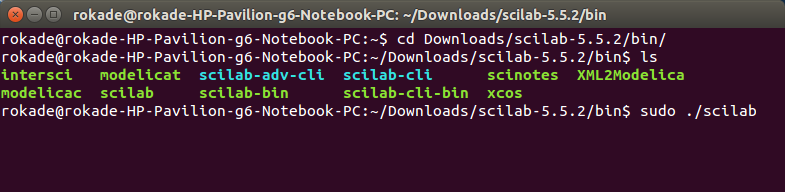
\includegraphics[scale=0.5]{\LocSWfig/linux-cd.png}
      \caption{Linux terminal to launch Scilab}
      \label{linux-cd}
\end{figure}

\subsection{Scilab-Arduino toolbox}
\label{sec:sci-ard-toolbox}
Scilab, by default, does not have the capability to connect to
Arduino. All such add-on functionalities are added to \scilab\ using
toolboxes. Just like we have different installation binaries of
\scilab\ for Windows and Linux, we have different toolboxes types for
Windows and Linux. \scilab-Arduino toolbox can be found inside
the {\tt Origin/tools/scilab/windows} or {\tt Origin/tools/scilab/linux} directory,
see \fnrefp{fn:file-loc}.  Use the one depending upon
which operating system you are using. The \scilab\ codes for various
experiments mentioned throughout this book can be found in {\tt
            Origin/user-code} directory. The {\tt user-code} directory will have
many sub-directories as per the experiments.

Let us now see how to load Scilab-Arduino toolbox. 
\begin{enumerate}
      \item First launch \scilab. On a Windows system, one may start/launch
            \scilab\ either through the Start menu or by double-clicking on the
            shortcut icon created on the Desktop. On a Linux system, one has to
            start \scilab\ through a terminal with root permissions, as
            explained in section \ref{scilab-installation-linux}.
      \item After launching \scilab, first we have to change the working
            directory. Below the menu bar, locate the tab called {\tt File Browser}. 
            Just below {\tt File Browser}, locate a folder-shaped icon. 
            This icon is used to {\tt Select a directory}. Click on this icon.   
            % click on the {\tt File} menu and then click on
            % the {\tt Change current directory} option as shown in
            % \figref{scilab-cd}.
            % \begin{figure}
            %       \centering
            %       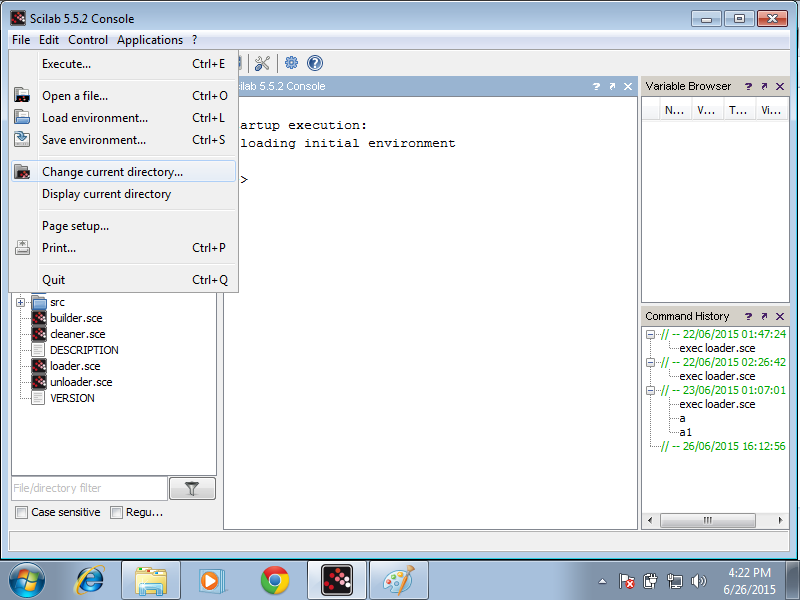
\includegraphics[width=\linewidth]{\LocSWfig/change-directory.png}
            %       \caption{Changing scilab directory}
            %       \label{scilab-cd}
            % \end{figure}
      \item Then, one has to browse to the toolbox folder
                  {\tt Origin/tools/scilab/windows} or {\tt Origin/tools/scilab/linux}, as the case
            may be, and click on, {\tt
                        Open}, as shown in \figref{scilab-browse}.
            \begin{figure}
                  \centering
                  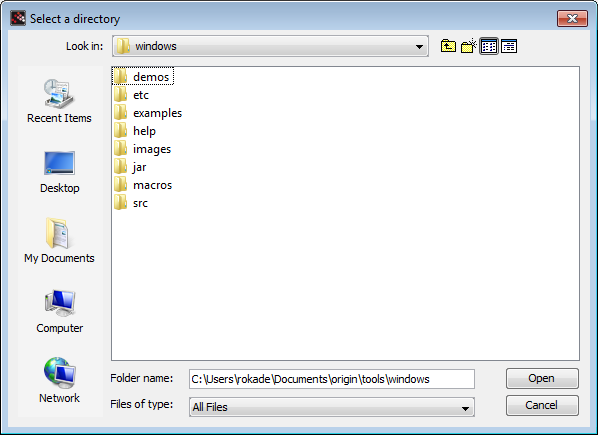
\includegraphics[width=\hgfig]{\LocSWfig/browse-directory.png}
                  \caption{Browsing toolbox directory}
                  \label{scilab-browse}
            \end{figure}
      \item After the previous step, the \scilab\ working directory becomes
            the toolbox folder.  See the {\tt file browser} panel on the
            left-hand side of the \scilab\ console, see \figref{builder}.  It
            will list out the contents of your current working directory. For a
            check, look for the file {\tt builder.sce}.  If you see this file,
            then you are in the right directory.
      \item Next, type the following command on the \scilab\ console: {\tt
            exec builder.sce} - this will build the toolbox and create a file
                  {\tt loader.sce}. This step has to be executed only the first
            time. The output of this step is illustrated in \figref{builder}.
            \begin{figure}
                  \centering
                  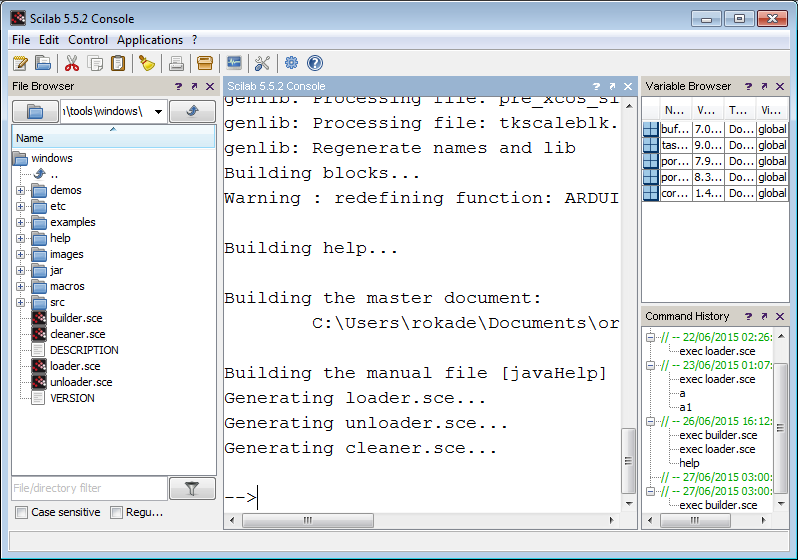
\includegraphics[width=\linewidth]{\LocSWfig/builder.png}
                  \caption{Output of builder.sce}
                  \label{builder}
            \end{figure}
      \item Next, type the command,
            {\tt exec loader.sce} -
            this will load the toolbox. This means all the new functions
            corresponding to the toolbox are loaded in the workspace. It
            will also make available new Xcos blocks, if any.  The
            output of this command is as shown in \figref{loader}.  If you clear
            the workspace for any reason, you will have to execute this command
            once again\footnote{Be careful
                  not to execute the {\tt clear} command.  This will clear the loaded
                  toolbox and you will have to execute the loader.sce file again.}.
            \begin{figure}
                  \centering
                  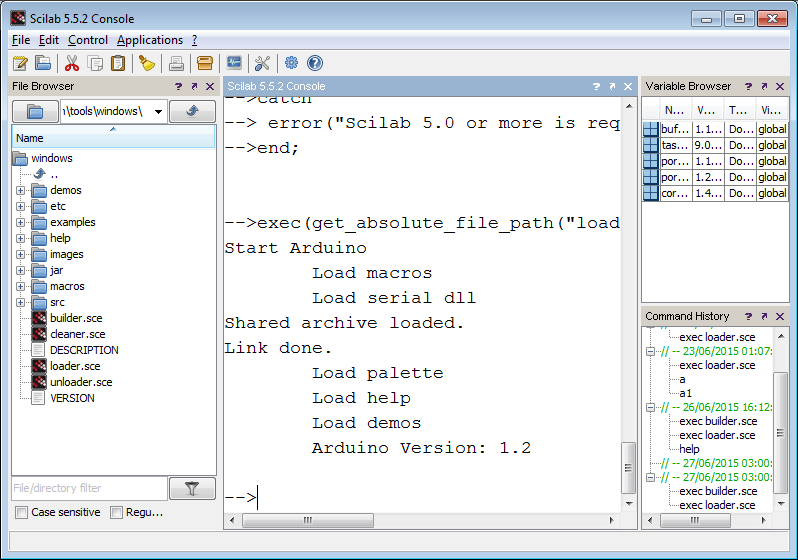
\includegraphics[scale=0.5]{\LocSWfig/loader.png}
                  \caption{Output of loader.sce}
                  \label{loader}
            \end{figure}
\end{enumerate}
The toolbox is now loaded and available for use. 

\subsection{Identifying Arduino communication port number}

Connect \arduino\ board to your computer. On a Windows system, doing
so for the first time will initiate the Windows device identification
routine. It may take a while before it finishes assigning a COM port
number to the \arduino\ board.  If Arduino IDE is installed using the
procedure outlined in \secref{arduino-ide}, required USB drivers for
Arduino get installed automatically.  Hence if you have installed the
Arduino IDE, it should not ask for drivers after you connect it.  As
usually Linux systems come with required drivers, the device is
automatically detected by the OS on connection.

Now let us see how to identify the COM port number. For a Windows
system, open the Device Manager. To do so, right-click on ``My
Computer'' and choose Properties. The Properties window that will open
will have Device Manager in the list on the left-hand side. In the
Device Manager window, look for ``Ports (COM and LPT)''. Double click on
it. It will show you the COM number for \arduino. 

\begin{figure}
      \centering
      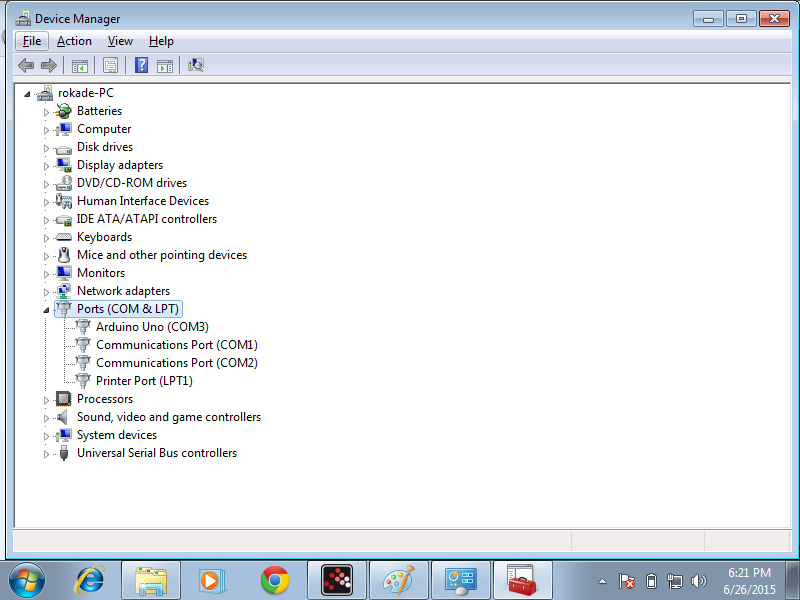
\includegraphics[width=\linewidth]{\LocSWfig/device-manager.png}
      \caption{Device Manager in windows}
      \label{dev-mgr}
\end{figure}

The result of the above exercise is shown in \figref{dev-mgr}.  In
this case, the system has detected Arduino with port number 3, which
appears as COM3.  In this book, we have taken the port for
communication as 2 and written code consistent with this assumption.    
As a result, we will now change it to
COM2\footnote{\label{fn:port}It is possible to leave it at whatever
      port number one gets.  It is also possible to choose any number
      between 2 and 99.  In this case, the port number should be
      changed accordingly in the code.  We will point this out throughout
      the book.}.  To change the port number, double click on the port
number. Its properties window will appear. Click on the ``Port
Settings'' tab and then click on ``Advanced'' button as shown in
\figref{com}.

\begin{figure}
      \centering
      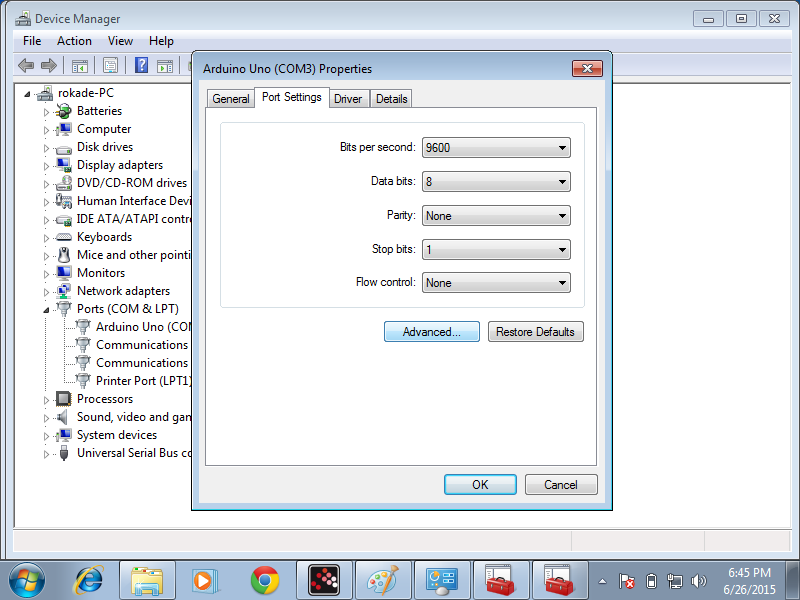
\includegraphics[scale=0.5]{\LocSWfig/com-properties.png}
      \caption{COM port properties window}
      \label{com}
\end{figure}

Click on the drop-down menu for COM port numbers. Choose the port
number COM2.  On clicking on ``OK'', Windows may warn you that the port
number is already in use. But given that you do not have any other USB
device connected you may force change it. Click on ``OK'' to close
all of the device manager windows. Now, we are set to go ahead with
port number 2. The stress on using port number 2 is just to be
consistent throughout the book. It is mainly for a beginner.

Now, let us see how to identify the port number on a Linux
system. Open a terminal by pressing Alt+Ctrl+T keys together. Then
type the following command and press enter, {\tt ls
            /dev/ttyACM*} -
the output of this command is shown in \figref{linux-port}. It has
detected the Arduino with the port number ``ttyACM0''.  The last character
in this string, namely 0, is the port number.  You may get 0 or a
number such as 1 or 2 in your case, for the port number.

\begin{figure}
      \centering
      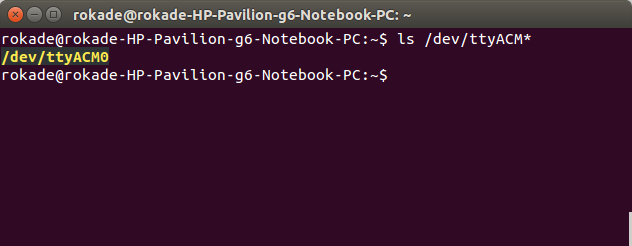
\includegraphics[scale=0.5]{\LocSWfig/linux-port.png}
      \caption{Port number on Linux terminal}
      \label{linux-port}
\end{figure}

\subsection{Testing Scilab-Arduino toolbox}
\label{sec:testing-scilab-arduino}
Now let us test the functioning of the toolbox. 
\begin{enumerate}
      \item Install Arduino IDE, as explained in \secref{sec:ard-start} and
            launch it.
      \item Read into the Arduino IDE, the firmware \ardref{ard:firmware}.
      \item Using the {\tt Upload} option of the Arduino IDE, load this
            firmware on to the \arduino\ board.
      \item Inside the {\tt Origin/tools/scilab} directory, locate a file {\tt
                        test\_firmware.sce}. This file will be used to test whether the
            firmware is properly installed.  This is an important step, as the
            connection between the computer and Arduino breaks down sometimes.
            Scilab-Arduino toolbox is unable to identify this difficulty - it has to
            be externally done.  If this difficulty is not identified and
            rectified, one will waste a lot of time and effort trying to debug
            the error.  This test has to be done in case of difficulties.
      \item In the \scilab\ console, type {\tt editor} and press the enter
            key. This will launch the editor. Click on ``File'' menu and choose
            ``Open''. Browse to the directory {\tt Origin/tools/scilab} and choose the
            file {\tt test\_firmware.sce}.  It will open
            \sciref{sci:test-firmware}.  
            %The \scilab\ editor with this file open is as shown in \figref{test-code}.
            %   \begin{figure}
            %     \centering
            %     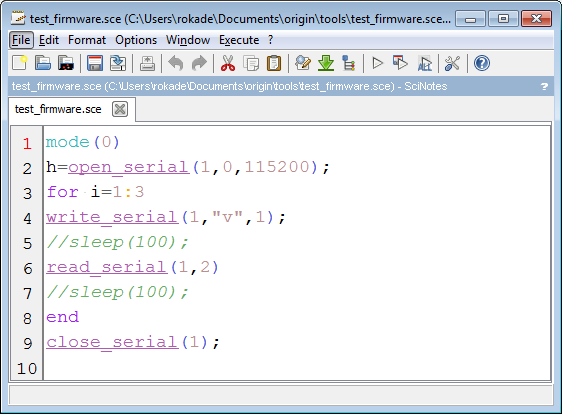
\includegraphics[scale=0.5]{\LocSWfig/test-code.png}
            %     \caption{Scilab code to test toolbox and firmware}
            %     \label{test-code}
            %   \end{figure}
            
      \item If you are using a Windows system and have set your port number
            as COM2, you need not make any changes to the file. Linux users,
            however, will mostly identify the port number as ``ttyACM0''. Hence, 
            they need to change the following line number
            \lstinputlisting[firstline=2,lastline=2]
            {\LocSWchkcode/test_firmware.sce}
            to
            \begin{lstlisting}[style=nonumbers]
  h = open_serial(1,0,115200); 
\end{lstlisting}
            
      \item To execute this code, on the menu bar, click on the {\tt
                        Execute}, option. Then choose {\tt File with no echo}. The output
            will appear on the Console as shown in \figref{test-console}.
            \begin{figure}
                  \centering
                  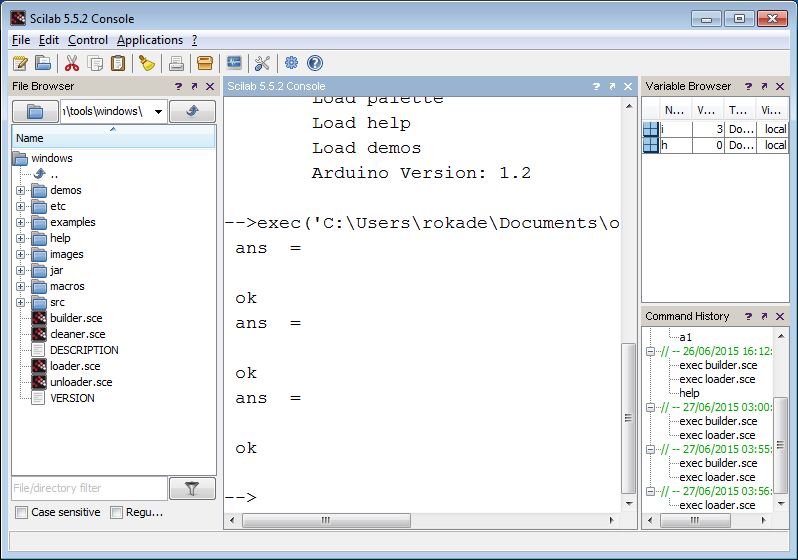
\includegraphics[scale=0.5]{\LocSWfig/test-console.png}
                  \caption{Scilab test code output}
                  \label{test-console}
            \end{figure}
            As shown in the figure, we see the response of this code as ``ans = '' and
            ``ok'' three times.  The
            code basically gives some input to Arduino three times and the
            program inside it returns ``ok'' three times.  This code thus confirms
            the working of Scilab-Arduino toolbox.  The code also confirms
            that the firmware inside the Arduino is correct.  It is alright if
            one or two of the attempts out of three give a blank response.  But
            all the three responses certainly should not be
            blank\footnote{\label{fn:firmware}If this step is unsuccessful,
                  one should check the connections and re-install the firmware}.
\end{enumerate}

Now let us take a look at the various functions facilitated by the
toolbox. The functions provided in the toolbox are as shown in 
\figref{func}. They are basically categorized into four categories:
configuration, digital, analog and motors. These functions will be
explained in detail in the subsequent chapters as and when they are
used.

\begin{figure}
      \centering
      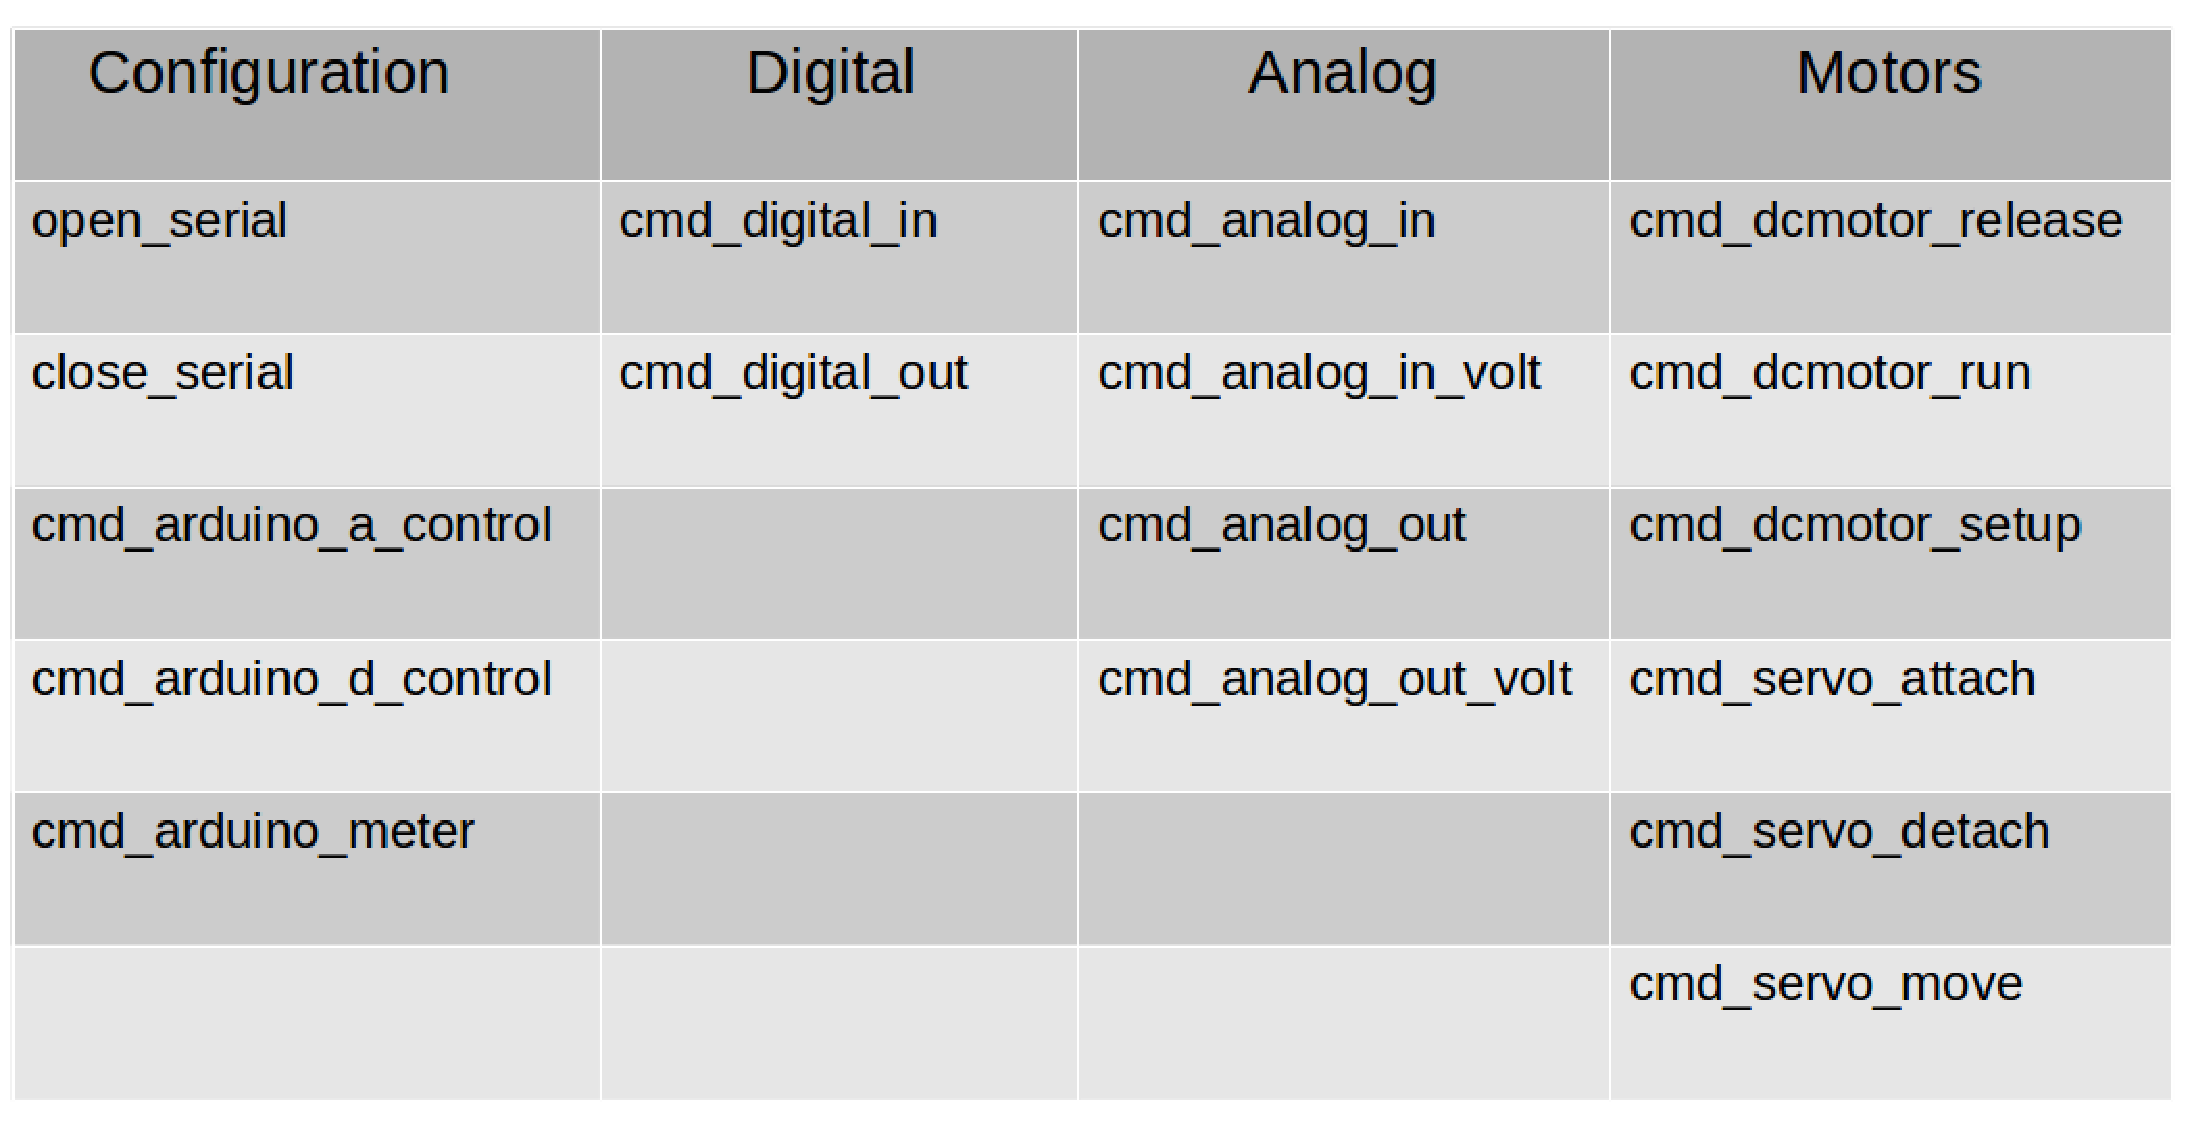
\includegraphics[width=\linewidth]{\LocSWfig/table_functions_crop.pdf}
      \caption{Arduino toolbox functions used in this book}
      \label{func}
\end{figure}

\subsection{Firmware}
\lstset{style=mystyle}
\label{sec:test-firmware-scilab}
\addtocontents{cod}{\protect\addvspace{\codclr}}
We have provided a Scilab code to check whether the firmware has been
properly installed.  That code is listed below.

\begin{scicode}
      \ccaption{A Scilab code to check whether the firmware is
            properly installed or not}{A Scilab code to check whether the
            firmware is properly installed or not.  Available at 
            \LocSWchkbrief{test\_firmware.sce}. Execute this code 
            by following the steps given in section 
            \ref{sec:testing-scilab-arduino}.}
      \label{sci:test-firmware}
      \lstinputlisting{\LocSWchkcode/test_firmware.sce}
\end{scicode}


\section{Xcos}
\label{sec:xcos-start}
Xcos is a graphical editor for \scilab\ \cite{xcos-ref}. Most of the
mathematical manipulations that can be done using \scilab\ scripts,
can be done using Xcos also.  The major advantage of Xcos is the
intuitive interface and easy connectivity across blocks. Xcos even
supports {\tt if else}, {\tt for}, and {\tt while} looping which forms
an integral part of any programming language. It is possible to code
the entire algorithm using Xcos blocks alone. It is also possible to
read from and write to the \scilab\ workspace through Xcos.

\subsection{Downloading, installing and testing}
Xcos comes pre-installed with \scilab. Hence a separate installation
of Xcos is not required. Let us explore the functionalities Xcos has
to offer. Xcos basically provides a graphical interface to \scilab.  

Xcos can be launched from \scilab\ by clicking on the Xcos icon
available on the \scilab\ menu bar. It can also be launched by simply
typing the command {\tt xcos} in the \scilab\ console. When Xcos is
launched, it will open a palette browser.  We have shown this in
\figref{sine-blk}, where we have selected a sine block.  At the time
of launch, Xcos will also open an empty canvas, called an untitled
Xcos window.

\begin{figure}
      \centering
      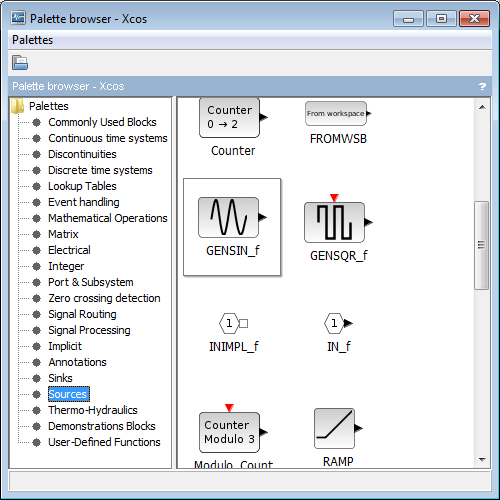
\includegraphics[width=\hgfig]{\LocSWfig/sine-blk.png}
      \caption{Sine generator in palette browser}
      \label{sine-blk}
\end{figure}

% \begin{figure}
% \centering
% 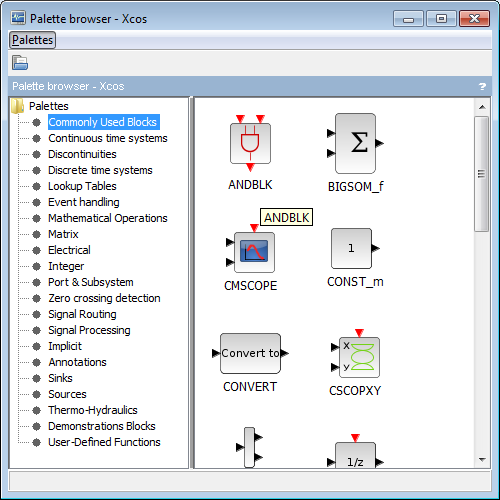
\includegraphics[scale=0.5]{\LocSWfig/palette-browser.png}
% \caption{Palette Browser}
% \label{palette}
% \end{figure}


% \begin{figure}
% \centering
% 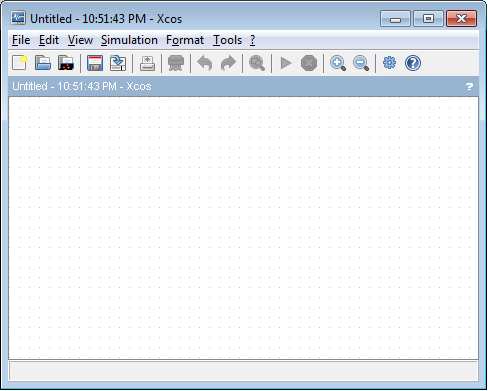
\includegraphics[scale=0.5]{\LocSWfig/untitled-xcos.png}
% \caption{Untitled Xcos window}
% \label{untitled}
% \end{figure}

Palette browser shows all of the available blocks that can be used. It
has been nicely categorized as per the functionality. For example,
blocks that generate signals/values without any input, fall under the
category {\tt Sources}. Similarly, blocks that take signals/values
without giving any output are categorized as {\tt Sinks}. This makes
finding a particular block very easy, specially when one does not know
the name of a block.

The untitled window is the one where one creates the Xcos
code/diagram. The relevant blocks have to be dragged and dropped from
the palette browser to the untitled window. The blocks are then
interconnected and configured as per the simulation, which we will
demonstrate next.

\subsection{Use case}
Let us build a simple Xcos simulation to plot a sine wave. This
simulation requires a sine wave source. It can be found in the {\tt
            Sources} category as shown in \figref{sine-blk}. Drag and drop this
block in the untitled Xcos window. 

Next, we need a block to plot the sine wave. A plotting block can be
found in the {\tt Sinks} category as shown in \figref{plot-blk}. The
name of this block is CSCOPE. Drag and drop this block in the untitled
Xcos window.  On the left-hand side, this block has an input port for
data.  It is black in colour, which may not be obvious in a black and
white printout.  The output from the sine block has to be connected
to this port.  At its top side, the CSCOPE block has another input
port, called an event port.  This is red in colour.  This port is used
to synchronize it with event generating devices.

\begin{figure}
      \centering
      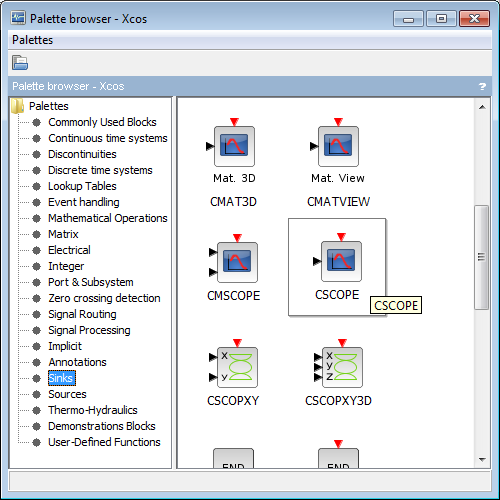
\includegraphics[width=\hgfig]{\LocSWfig/plot-blk.png}
      \caption{CSCOPE block in xcos}
      \label{plot-blk}
\end{figure}

As the CSCOPE block has an
input event port, we need a source that generates events. Hence, the
next block that we need is an event generator block and it can be
found in the {\tt Sources} category. This is illustrated in figure
\ref{clk-blk}. The name of this block is CLOCK\_c. Drag and drop this
block in the untitled Xcos window.

\begin{figure}
      \centering
      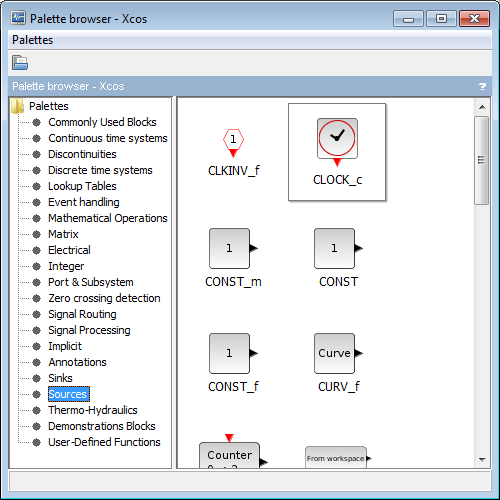
\includegraphics[width=\hgfig]{\LocSWfig/clock-blk.png}
      \caption{CLOCK\_c block in xcos}
      \label{clk-blk}
\end{figure}

The next step is to interconnect the blocks together. A black color
port can only be connected to another black color port. A black color
port cannot be connected to a red color port and vice versa.  That is,
a data port cannot be connected to an event port.  Linking
two blocks is a bit crucial and may need a few attempts before one gets
comfortable. To link two blocks, first click and hold the left mouse
button over the output port of the source block. Without releasing the
mouse button, touch the mouse pointer to the input port of the sink
block. If a connection is possible there, the port will turn
``green''. At this point, release the mouse button and the blocks should
get connected. Follow this procedure and complete the connection as
shown in \figref{sine-gen}.  Save this file with the name {\tt
            sine-generator}.  

\begin{figure}
      \centering
      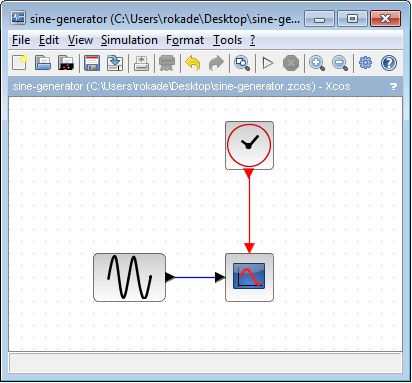
\includegraphics[width=\smfig]{\LocSWfig/sine-gen.png}
      \caption{Sine generator in Xcos}
      \label{sine-gen}
\end{figure}

Let us simulate this Xcos code. On the menu bar, click on the {\tt
            Simulation} menu and choose {\tt Start}. You will get a graphic
window with a running sine wave as shown in \figref{sine-output}.

\begin{figure}
      \centering
      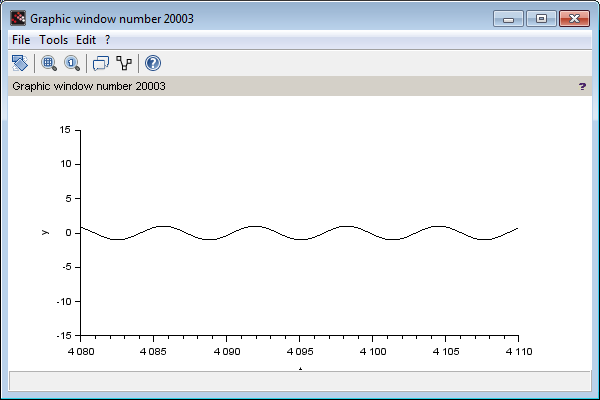
\includegraphics[width=\lgfig]{\LocSWfig/sine-output.png}
      \caption{Sine generator Xcos output}
      \label{sine-output}
\end{figure}

This is because we are running the simulation using the default
configuration.  We would like a stationary plot.  If the simulation is
still running, go to the Simulation menu and choose Stop.  Double
click on the CSCOPE block. Its properties window will appear as shown
in \ref{cscope-config}. Note the value of the {\tt Refresh period}. It
is by default 30. Click on Ok.

\begin{figure}
      \centering
      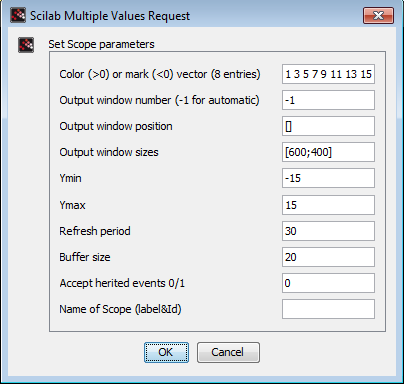
\includegraphics[width=\lgfig]{\LocSWfig/cscope-config.png}
      \caption{CSCOPE configuration window}
      \label{cscope-config}
\end{figure}

Next, on the menu bar, click on the {\tt Simulation} menu and choose
      {\tt Setup}. The {\tt Set Parameters} window will open. The first
parameter is {\tt Final integration time}. It decides for how long the
simulation will run. Change it to be equal to the {\tt Refresh period}
of the CSCOPE block.  That is, change it to 30 as shown in
\figref{sim-setup}. Now start the simulation and you will get a static
plot.  Other paramenters of blocks can also be changed. For example,
one may want to change the input amplitude/frequency or change the
plot scales, etc. All these are left to the reader to explore.

\begin{figure}
      \centering
      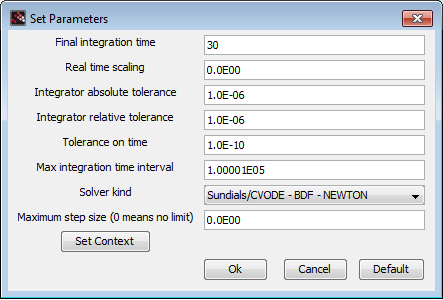
\includegraphics[width=\lgfig]{\LocSWfig/sim-setup.png}
      \caption{Simulation setup window}
      \label{sim-setup}
\end{figure}

Although we have demonstrated a very basic level of Xcos simulation,
this idea can be used for complex processes as well.  Using Xcos, it
is possible to have user-defined blocks. The user can code the
working of the block as a function in \scilab\ script and then call it
from Xcos.  It is also possible to create subsystems.  
One can even read from and write to C binaries.  Xcos comes with
several pre-defined libraries and hence, it is possible to carry out
other kinds of simulation, such as electrical circuit simulation and
basic thermo-hydraulic simulation, for example.  A detailed 
explanation and demonstration are beyond the scope of this book.


\subsection{Xcos-Arduino}
\scilab-Arduino toolbox not only provides functions to be used in
\scilab\ scripts but also provides new Arduino-specific blocks. As
shown in \figref{arduino-palette} new Arduino blocks are now available
for use.  Similar to the categorization of the functions, the Xcos
blocks are also categorized as configuration, digital, analog and
motors. Again, it is possible to conduct the experiments only using
Xcos. Xcos codes for every experiment are provided throughout the
book. The Arduino blocks can be easily connected to Xcos native
blocks. A detailed block help for every block can be sought by right-clicking on the block and choosing ``Block help''. This is illustrated
in \figref{blk-help}.

\begin{figure}
      \centering
      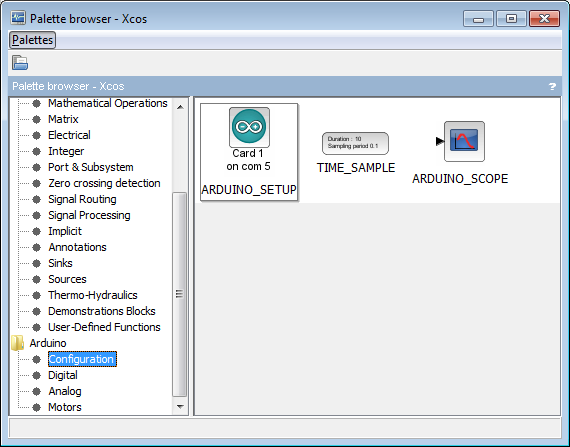
\includegraphics[width=\lgfig]{\LocSWfig/arduino-palette.png}
      \caption{Palette browser showing Arduino blocks}
      \label{arduino-palette}
\end{figure}

\begin{figure}
      \centering
      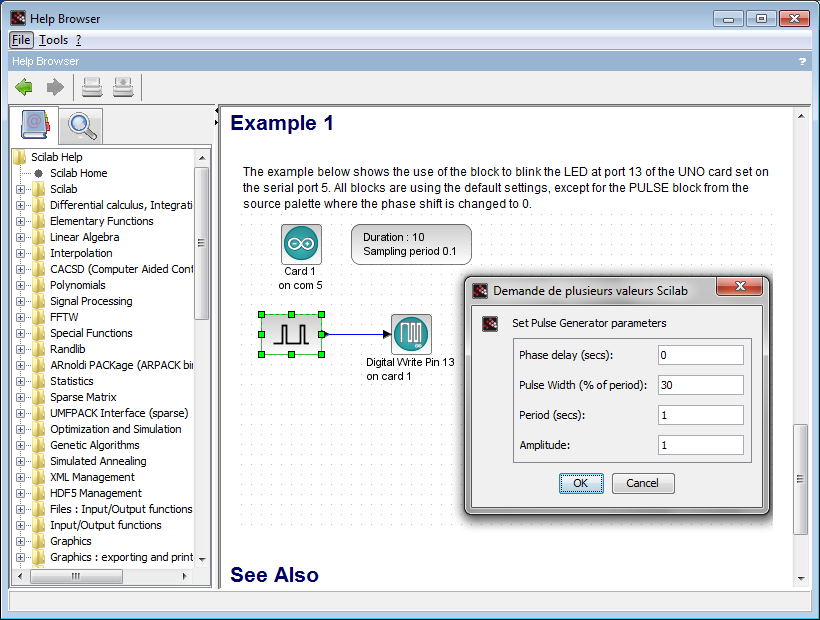
\includegraphics[width=\lgfig]{\LocSWfig/xcos-help.png}
      \caption{Xcos block help}
      \label{blk-help}
\end{figure}
